%!TEX root = main.tex
\chapter{Implementation}
% In many cases, you will not be able to realize the full design. Often the implementation is only a demonstrator of ideas. 
% It is therefore important that you focus on the most important aspects of your system (depending on research questions). 
% In the report you have to justify the choices that are done.
In this chapter we will go through the implementations made in order to develop the PeacefulBanana tool, and the rationale behind the decisions made. 

Below you can see an overview of the entire system design, it was designed so the users can see the data tailored to their team and work.

\begin{figure}[h!]
    \centering
        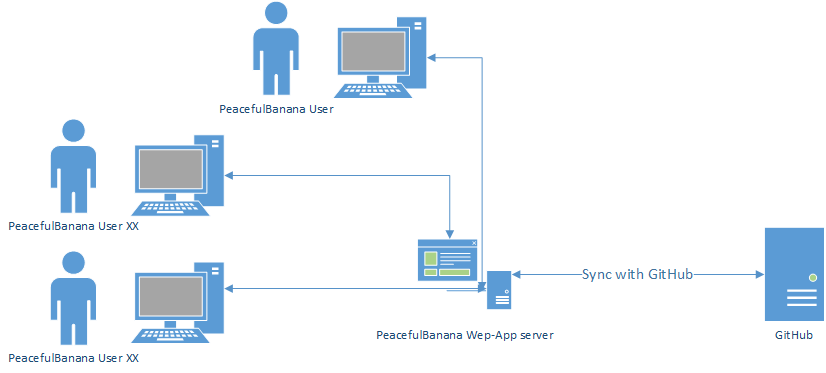
\includegraphics[width=0.8\textwidth]{Clientservergithub}
    \caption{Overview of system design.}
    \label{ClientServerGithub}
\end{figure}

\section{Server}
When choosing a framework for the prototype, several alternatives where discussed and their architecture was a vital part of the selection. Based on these criterias the server was implemented with Grails a framework for web applications, it is better described in the section following.

\subsection{Grails}
\begin{figure}[h!]
\centering
    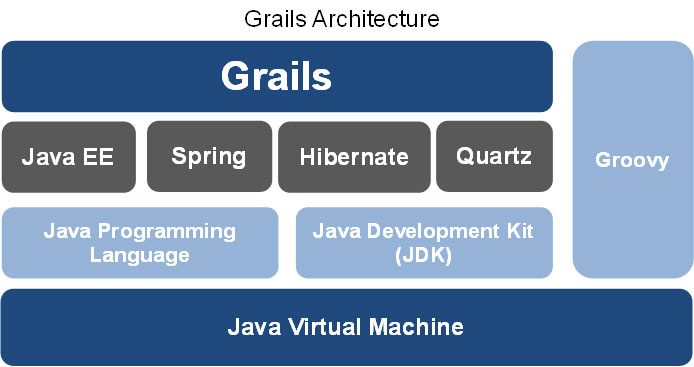
\includegraphics[width=0.8\textwidth]{Grails-Architecture}
\caption{Overview of Grails architecture.}
\end{figure}

Grails is an open source web application framework which uses the programming language Groovy(which is buildt on top of the Java Virtual Machine). When Grails was developed, it's developers aimed to re-use proven technologies such as Hibernate, Spring etc. 
\begin{figure}[h!]
    \centering
        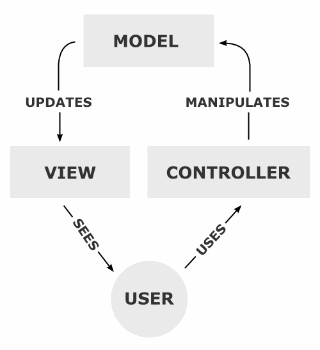
\includegraphics[width=0.8\textwidth]{MVC}
    \caption{Model-view-controller paradigm}
\end{figure}
It uses a MVC\footnote{Model View Controller} pattern, where it changes a gsp-file(Groovy server page), these files represents the different views related to each controller. The data retrieved by the controller from the database.


\section{Database}
In this section we will show how the database is designed, the diagram below shows the relationship between the differet data-types. The datatypes have been categorised regarding to their origin and are discussed later in this section.

\begin{figure}[h!]
\centering
	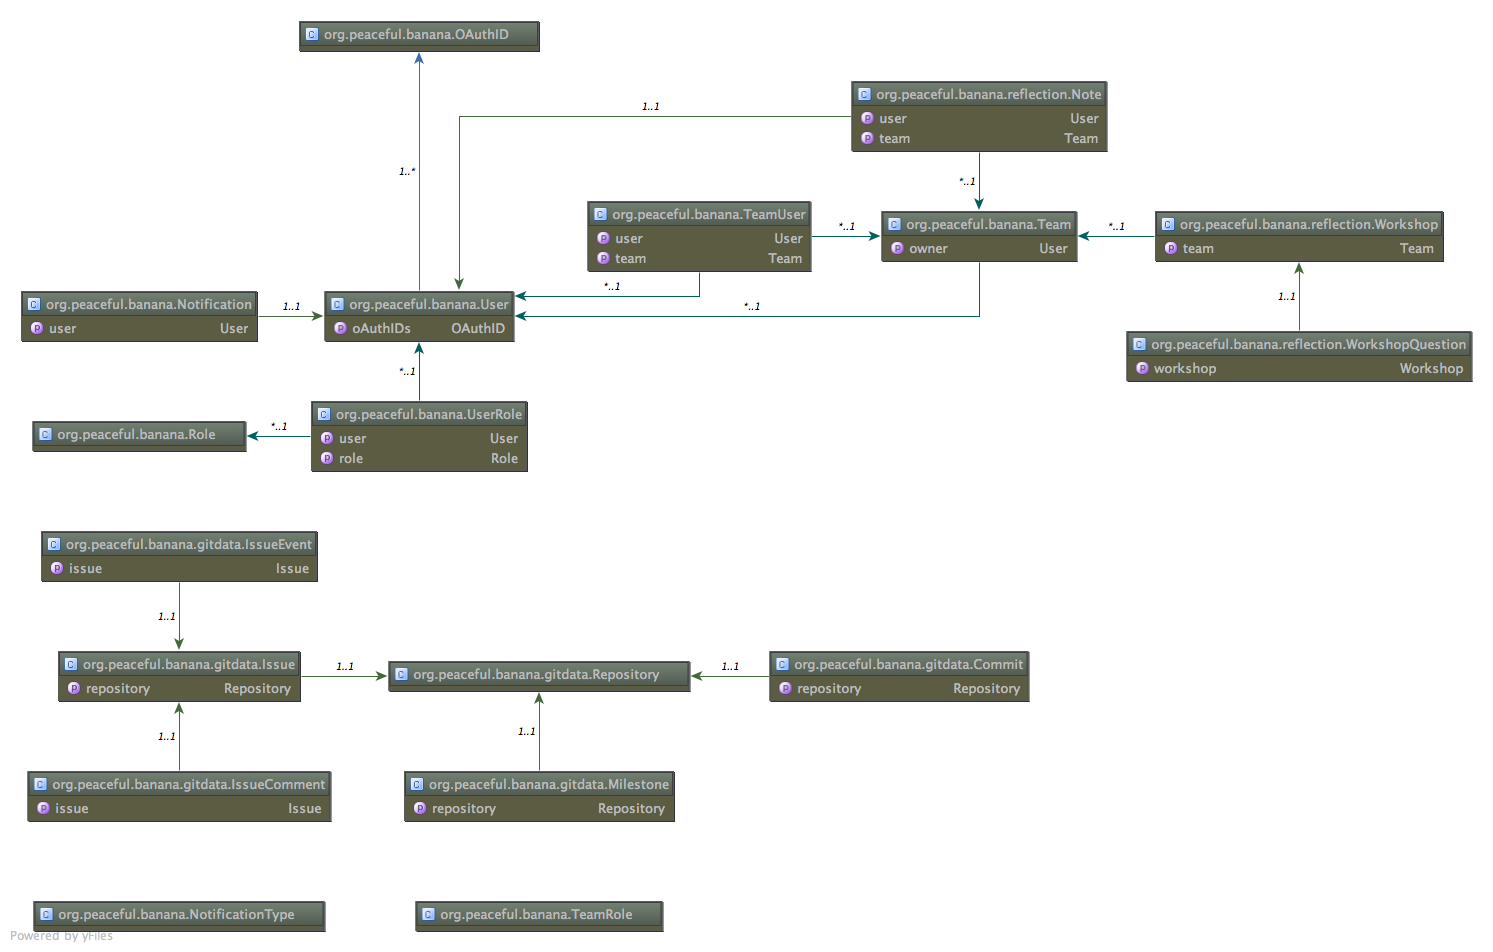
\includegraphics[width=\textwidth]{databaseDomainDiagram}
\caption{Domain diagram, shows the relationship between different classes.}
\label{databaseDomainDiagram}
\end{figure}

\subsection{User data}
In this section we will show and discuss all data stored related to users, the tables below is r \\

\subsubsection*{User}
In this table general data is stored about each user and field relevant to authenticate them.

The password are encrypted with SHA-512 encryption.\\

\vspace{0.5cm}
\begin{tabularx}{\linewidth}{| c | X |}
    \hline
    \rowcolor[gray]{0.8}
    \textbf{Field} & \textbf{Description} \\
    \hline
    Id & Unique generated when the user is first created\\ \hline
    UserName & This field stores the users username\\ \hline
   	Password & This field stores the users password as a encrypted string, the password is encryptet with SHA-512 encryption\\ \hline
    Email & This field stores the users email\\ \hline
    FirstName & This field stores the users first name\\ \hline
    LastName & This field stores the users last name\\ \hline
    SelectedRepo & The GitHub generated id of the repository currently selected by the user\\ \hline
    GitLogin & The users GitHub login, used to bind commits to the user\\ \hline
    DateCreated & This field stores the date when the user was first created\\
    \hline
\end{tabularx}
\vspace{0.5cm}

\subsubsection*{Role}
The different roles that the users can be assigned to. These are hierarchy so that the highest gains access to the subset of this access level. \\

\vspace{0.5cm}
\begin{tabularx}{\linewidth}{| c | X |}
    \hline
    \rowcolor[gray]{0.8}
    \textbf{Field} & \textbf{Description} \\
    \hline
    Id & Unique generated when the role is first created.\\ \hline
    Authority & This field contains the level of authority.\\
    \hline
\end{tabularx}
\vspace{0.5cm}

\subsubsection*{UserRole}
Both fields in this table are combined for the primary key such that each role can only be given to each user once. \\

\vspace{0.5cm}
\begin{tabularx}{\linewidth}{| c | X |}
    \hline
    \rowcolor[gray]{0.8}
    \textbf{Field} & \textbf{Description} \\
    \hline
    User & Foreign key for the user\\ \hline
    Role & Foreign key for the role \\
    \hline
\end{tabularx}
\vspace{0.5cm}

\subsubsection*{Notification}
Notifications are used to prompt users about reflection sessions and such. \\

\vspace{0.5cm}
\begin{tabularx}{\linewidth}{| c | X |}
    \hline
    \rowcolor[gray]{0.8}
    \textbf{Field} & \textbf{Description} \\
    \hline
    Id & Unique generated when the notification is first created\\ \hline
    Title & This field stores the title\\ \hline
   	Body & This field stores the entire message.\\ \hline
    DateCreated & Timestamp generated when the notification is first created.\\ \hline
    Unread & Variable to state if the message is read.\\ \hline
    Cleared & Variable to state if the message is cleared or not.\\ \hline
    NotificationType & The notification type, possible types are 'Reflection' or 'Other'.\\ \hline
    User & A forreign key to the user that received the notification.\\ 
    \hline
\end{tabularx}
\vspace{0.5cm}

\subsection{Github data}
Github data is stored localy to enhance performance. During initial testing it was discovered that polling github.com for data each time it was needed, made the application very slow and put unnecessary stress on the github servers. The following data-types where therefor storred localy.

\subsubsection*{Milestones}
Milestones are major goals consisting of several minor goals called issue, with or without a due date. \\

\vspace{0.5cm}
\begin{tabularx}{\linewidth}{| c | X |}
    \hline
    \rowcolor[gray]{0.8}
    \textbf{Field} & \textbf{Description} \\
    \hline
    GithubId & Unique id from github.com\\ \hline
    Name & The milestones name.\\ \hline
   	Description & A description of the milestone, like what features is to be implemented.\\ \hline
    Status & A variable to say if its open or closed.\\ \hline
    CreatedDate & The timestamp which the milestone is created.\\ \hline
    DueDate & A date which the milestone is due on. This is null if the milestone does not got a due date.\\ \hline
    ClosedDate & A timestamp when the milestone is closed.\\ 
    \hline
\end{tabularx}
\vspace{0.5cm}

\subsubsection*{Issues}
Issues are minor goals or bugs, these issues can be bould to a milestone or independent. \\

\vspace{0.5cm}
\begin{tabularx}{\linewidth}{| c | X |}
    \hline
    \rowcolor[gray]{0.8}
    \textbf{Field} & \textbf{Description} \\
    \hline
    GithubId & Unique id from github.com\\ \hline
    Name & The issues name.\\ \hline
   	Body & A description of the milestone, like what features is to be implemented.\\ \hline
    State & A variable to say if its open or closed.\\ \hline
    Number & A number unique to the repository which is used for refering the issue in the commit messages.\\ \hline
    Repository & A forreign key to the repository it is bound to.\\ \hline
    MilestoneNumber & The milestone which the issue is bound to.\\ \hline
    CreatedAt & The timestamp which the milestone is created.\\ \hline
    UpdatedAt & The timestamp which the milestone last was updated.\\ 
    \hline
\end{tabularx}
\vspace{0.5cm}

\subsubsection*{Commits}
At any given time a developer changes something in the sourcecode it can be commited to the version controll system, in this case git/github. These are the commits we store and use for reflection. \\

\vspace{0.5cm}
\begin{tabularx}{\linewidth}{| c | X |}
    \hline
    \rowcolor[gray]{0.8}
    \textbf{Field} & \textbf{Description} \\
    \hline
    GithubId & Unique id from github.com\\ \hline
    Message & The commit message which we gather tags from, these tags are marked hashtags.\\ \hline
   	Login & The github user which did the commit.\\ \hline
    CreatedDate & The timestamp which the commit is created.\\ \hline
    Additions & A date which the milestone is due on. This is null if the milestone does not got a due date.\\ \hline
    Deletions & A timestamp when the milestone is closed.\\ \hline
    Total & A total of lines in the commit.\\
    \hline
\end{tabularx}
\vspace{0.5cm}

\subsubsection*{Repository}
The current data is storred about each repository, in the corresponding fields in the table bellow. \\

\vspace{0.5cm}
\begin{tabularx}{\linewidth}{| c | X |}
    \hline
    \rowcolor[gray]{0.8}
    \textbf{Field} & \textbf{Description} \\
    \hline
    GithubId & Unique id from github.com\\ \hline
    Name & The repositorys name.\\ \hline
   	Description & A description of the repository.\\ \hline
    CreatedAt & The timestamp which the commit is created.\\ \hline
    UpdatedAt & The timestamp recorded when the milestone last was updated.\\ 
    \hline
\end{tabularx}
\vspace{0.5cm}

\subsection{Collaboration data}
Teams are bound uniquelie to a repositorie, each repository will only have one team bound to it and every user with access(being a contributor) to the repository on Github will have the possibility to join the team.  \\%%Every user with access to the prepository on Github will see this team.%%
\subsubsection*{Team}
These teams are bound to a repository and there can only be one not created for each team by a user each day. \\

\vspace{0.5cm}
\begin{tabularx}{\linewidth}{| c | X |}
    \hline
    \rowcolor[gray]{0.8}
    \textbf{Field} & \textbf{Description} \\
    \hline
    Id & Unique id generated when the team is created.\\ \hline
   	Owner & A forreign key to the user that created the team.\\ \hline
   	Name & The teams name.\\ \hline
    Repository & The githubId of the repository bound to the team.\\ 
    \hline
\end{tabularx}
\vspace{0.5cm}

\subsubsection*{TeamUser}
The users attached to the team. \\

\vspace{0.5cm}
\begin{tabularx}{\linewidth}{| c | X |}
    \hline
    \rowcolor[gray]{0.8}
    \textbf{Field} & \textbf{Description} \\
    \hline
    UserId & A forreign key to the user.\\ \hline
   	TeamId & A forreign key to the team.\\ \hline
   	Role & The users role in the team. There are possible roles are 'Manager' and 'Developer'\\ \hline
    Active & A variable that states if the user has selected this team as his active. Only one can be active per user at any given time.\\ 
    \hline
\end{tabularx}
\vspace{0.5cm}

\subsection{Reflection data}
\subsubsection*{Notes}
These notes are bound to a team and there can only be created one for each team by a user each day. \\

\vspace{0.5cm}
\begin{tabularx}{\linewidth}{| c | X |}
    \hline
    \rowcolor[gray]{0.8}
    \textbf{Field} & \textbf{Description} \\
    \hline
    Id & Unique id generated when the note is created.\\ \hline
    Team & A forreign key to the team the note is bound to.\\ \hline
   	User & A forreign key to the user that created the note.\\ \hline
   	Mood & A level regarding the current mood the user that created the note recorded for that day. Mood is recoreded as a number between 1-100 where 100 is very happy and 1 is very sad.\\ \hline
   	Contribution & The top 2 contributions done that day for the team by the user.\\ \hline
   	Improvements & The 2 things that can be improved by the user that day for the team.\\ \hline
   	Shared & Variable that states that the note is shared with the team.\\ \hline
    CreatedAt & The timestamp which the commit is created.\\ \hline
    UpdatedAt & The timestamp recorded when the milestone last was updated.\\ 
    \hline
\end{tabularx}
\vspace{0.5cm}

\subsubsection*{Workshop}
Managers or owners of teams can create reflection workshops, where it is generated a set of questions based on the tags used by the teams members in the selected periode. \\

\vspace{0.5cm}
\begin{tabularx}{\linewidth}{| c | X |}
    \hline
    \rowcolor[gray]{0.8}
    \textbf{Field} & \textbf{Description} \\
    \hline
    Id & Unique id generated when the workshop is created.\\ \hline
   	TeamId & A forreign key to the team.\\ \hline
   	CreatedAt & The timestamp which the workshop is created.\\ \hline
   	DurationStart & The timestamp which the workshop periode starts.\\ \hline
   	DateStart & The timestamp which the workshop periode ends.\\ 
    \hline
\end{tabularx}
\vspace{0.5cm}

\textbf{WorkshopQuestions}
This table holds the questions generated from the commit messages. \\

\vspace{0.5cm}
\begin{tabularx}{\linewidth}{| c | X |}
    \hline
    \rowcolor[gray]{0.8}
    \textbf{Field} & \textbf{Description} \\
    \hline
    Id & Unique id generated when the question is created.\\ \hline
   	Workshop & A forreign key to the workshop.\\ \hline
   	QuestionText & The generated question.\\ \hline
   	CommitTag & The tag which the question is generated from.\\ 
    \hline
\end{tabularx}
\vspace{0.5cm}

\section{User Interface}
When designing the Peaceful Banana, it was clear that our task required a lot of design work. In order to create a simple yet informative page-layout the twitter boostrap framework was chosen.

The design itself is heavily based on the fluid layout and sign in examples from the official examples.

\subsection{Twitter bootstrap}
%Tell something about twitter bootstrap and why/how we used it.
Twitter boostrap is a front-end framework for easier and faster web development, it is widely used and makes it possible to create beautiful webpages without much work. Bootstrap utilizes both ofs the HTML5 and CSS3 standards.

\subsection{jQuery}
It was initally released under the MIT licence in 2006 to make it easier to select DOM\footnote{Document-Object-Model} objects and create powerful dynamic web pages and applications.

JQuery has been used for AJAX\footnote{Asynchronous JavaScript and XML}, this is a way to change the contents DOM objects asynchronous from javascript.

\subsubsection{AwesomeCloud}
Awesome cloud is a plugin for jQuery for creating a tagcloud, it retrieves data from DOM-objects and renderes them as a cloud where the font-size increases with the occurence of tags, the tagcloud is then drawn on the HTML5 canvas.
